\documentclass[tikz,border=4pt]{standalone}
\usepackage{tikz}
\usetikzlibrary{positioning,shapes.geometric,shapes.symbols,arrows.meta,fit,calc,backgrounds}

\definecolor{ctrlFill}{HTML}{dae8fc}
\definecolor{ctrlStroke}{HTML}{6c8ebf}
\definecolor{memFill}{HTML}{ffe6cc}
\definecolor{memStroke}{HTML}{d79b00}
\definecolor{calcFill}{HTML}{cce5ff}
\definecolor{calcStroke}{HTML}{4a86e8}
\definecolor{dataFill}{HTML}{d5e8d4}
\definecolor{dataStroke}{HTML}{82b366}
\definecolor{newStroke}{HTML}{b85450}
\definecolor{dramFill}{HTML}{f2f2f2}
\definecolor{dramStroke}{HTML}{666666}
\definecolor{pkrnCol}{HTML}{c44b3a}
\definecolor{hubFill}{HTML}{f8cecc}
\definecolor{hubStroke}{HTML}{b85450}

\begin{document}
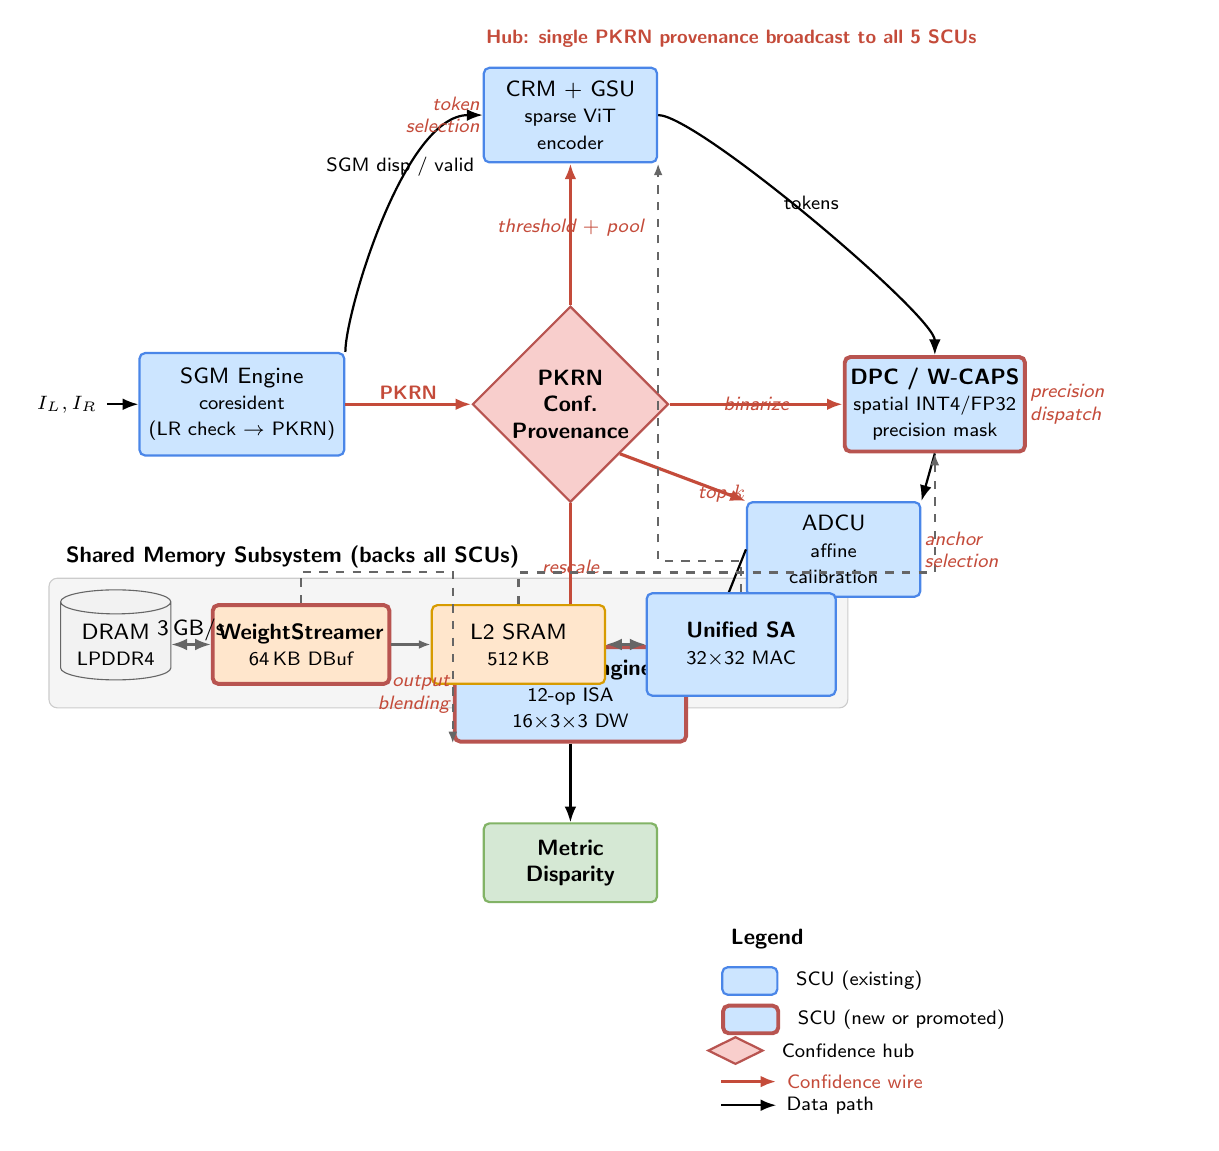
\begin{tikzpicture}[
  font=\footnotesize\sffamily,
  node distance=3mm,
  stage/.style={draw=calcStroke, fill=calcFill, rounded corners=2pt, thick, minimum width=26mm, minimum height=13mm, align=center, inner sep=2pt},
  newstage/.style={draw=newStroke, fill=calcFill, rounded corners=2pt, line width=0.5mm, minimum width=26mm, minimum height=13mm, align=center, inner sep=2pt},
  mem/.style={draw=memStroke, fill=memFill, rounded corners=2pt, thick, minimum width=22mm, minimum height=10mm, align=center, inner sep=2pt},
  newmem/.style={draw=newStroke, fill=memFill, rounded corners=2pt, line width=0.5mm, minimum width=22mm, minimum height=10mm, align=center, inner sep=2pt},
  dram/.style={draw=dramStroke, fill=dramFill, cylinder, shape border rotate=90, aspect=0.25, minimum height=10mm, minimum width=14mm, align=center},
  outp/.style={draw=dataStroke, fill=dataFill, rounded corners=2pt, thick, minimum width=22mm, minimum height=10mm, align=center, inner sep=2pt, font=\footnotesize\sffamily\bfseries},
  hub/.style={draw=hubStroke, fill=hubFill, diamond, thick, minimum width=22mm, minimum height=16mm, align=center, inner sep=1pt, font=\footnotesize\sffamily\bfseries},
  scu/.style={draw=calcStroke, fill=calcFill, rounded corners=2pt, thick, minimum width=22mm, minimum height=12mm, align=center, inner sep=2pt},
  newscu/.style={draw=newStroke, fill=calcFill, rounded corners=2pt, line width=0.5mm, minimum width=22mm, minimum height=12mm, align=center, inner sep=2pt},
  arr/.style={-{Latex[length=2mm]}, thick},
  pkrnarr/.style={-{Latex[length=2mm]}, thick, draw=pkrnCol, line width=0.4mm},
  pkrndash/.style={-{Latex[length=2mm]}, draw=pkrnCol, line width=0.35mm, dashed},
  membus/.style={-{Latex[length=1.5mm]}, thick, draw=dramStroke},
  lbl/.style={font=\footnotesize\sffamily, inner sep=1pt},
  xflbl/.style={font=\scriptsize\sffamily\itshape, text=pkrnCol, inner sep=1pt},
  plbl/.style={font=\scriptsize\sffamily\bfseries, text=pkrnCol, inner sep=1pt}
]

% ============================================================
% LEFT: SGM producing the confidence provenance
% ============================================================
\node[stage] (sgm) at (0,0) {SGM Engine\\\scriptsize coresident\\\scriptsize (LR check $\to$ PKRN)};

% ============================================================
% CENTER: CONFIDENCE PROVENANCE HUB
% ============================================================
\node[hub, right=16mm of sgm] (hub) {PKRN\\Conf.\\Provenance};

% ============================================================
% FOUR SPOKES: SCUs arranged around the hub
% Each SCU shows: name + module-local transform annotation
% ============================================================

% Top spoke: CRM + GSU (token selection stage)
\node[scu, above=18mm of hub] (crmgsu) {CRM $+$ GSU\\\scriptsize sparse ViT\\\scriptsize encoder};
\node[xflbl] (tr1) at ($(hub.north)!0.55!(crmgsu.south)$) {threshold $+$ pool};

% Right-top spoke: DPC / W-CAPS (decoder precision)
\node[newscu, right=22mm of hub] (dpc) {\textbf{DPC / W-CAPS}\\\scriptsize spatial INT4/FP32\\\scriptsize precision mask};
\node[xflbl] (tr2) at ($(hub.east)!0.5!(dpc.west)$) {binarize};

% Right-bottom spoke: ADCU (calibration)
\node[scu, below right=6mm and 16mm of hub] (adcu) {ADCU\\\scriptsize affine\\\scriptsize calibration};
\node[xflbl, above=-0.2mm of adcu.north west, anchor=south east, inner sep=0pt] {top-$k$};

% Bottom spoke: FU / FE-v2 (output fusion)
\node[newscu, below=18mm of hub] (fe) {\textbf{FU / FusionEngineV2}\\\scriptsize 12-op ISA\\\scriptsize 16$\times$3$\times$3 DW};
\node[xflbl] (tr4) at ($(hub.south)!0.45!(fe.north)$) {rescale};

% ============================================================
% CONFIDENCE PROVENANCE FAN-OUT (red bold arrows to 4 SCUs)
% ============================================================
\draw[pkrnarr] (sgm.east) -- node[plbl, above]{PKRN} (hub.west);
\draw[pkrnarr] (hub.north) -- (crmgsu.south);
\draw[pkrnarr] (hub.east)  -- (dpc.west);
\draw[pkrnarr] (hub.south east) -- (adcu.north west);
\draw[pkrnarr] (hub.south) -- (fe.north);

% ============================================================
% DATA PATH (solid black arrows: stereo pair -> SGM -> SCUs -> output)
% ============================================================
% Input L,R images feeding SGM
\node[left=4mm of sgm, font=\scriptsize\sffamily] (inp) {$I_L, I_R$};
\draw[arr] (inp) -- (sgm.west);

% SGM -> disparity flow bypassing hub: feeds sparse-encoder (CRM/GSU) + fusion (FE)
\coordinate (sgmout) at ($(sgm.east)+(0,5mm)$);
\draw[arr] (sgm.north east) .. controls +(0,5mm) and +(-10mm,0) .. (crmgsu.west)
  node[pos=0.6, above, font=\scriptsize\sffamily] {SGM disp / valid};

% Encoder output feeds decoder (DPC/W-CAPS), then ADCU, then FE
\draw[arr] (crmgsu.east) .. controls +(5mm,0) and +(0,5mm) .. (dpc.north)
  node[pos=0.5, above, font=\scriptsize\sffamily] {tokens};
\draw[arr] (dpc.south) -- (adcu.north east);
\draw[arr] (adcu.west) -- (fe.east);

% Output
\node[outp, below=10mm of fe] (outn) {Metric\\Disparity};
\draw[arr] (fe.south) -- (outn.north);

% ============================================================
% BOTTOM: Memory subsystem row
% ============================================================
\node[dram,   below=22mm of inp, anchor=north west] (dram) {DRAM\\\scriptsize LPDDR4};
\node[newmem, right=5mm of dram] (ws)              {\textbf{WeightStreamer}\\\scriptsize 64\,KB DBuf};
\node[mem,    right=5mm of ws]   (l2)              {L2 SRAM\\\scriptsize 512\,KB};
\node[stage,  right=5mm of l2, minimum width=24mm] (sa) {\textbf{Unified SA}\\\scriptsize 32$\times$32 MAC};

\begin{pgfonlayer}{background}
  \node[fit=(dram)(sa), fill=gray!8, rounded corners=3pt, inner sep=4pt, draw=gray!40] (membox) {};
\end{pgfonlayer}
\node[anchor=south west, font=\footnotesize\sffamily\bfseries] at ($(membox.north west)+(1mm,0mm)$) {Shared Memory Subsystem (backs all SCUs)};

% Memory arrows
\draw[membus, {Latex[length=2mm]}-{Latex[length=2mm]}] (dram.east) -- node[lbl, above]{3\,GB/s} (ws.west);
\draw[membus] (ws.east)  -- (l2.west);
\draw[membus, {Latex[length=2mm]}-{Latex[length=2mm]}] (l2.east)  -- (sa.west);

% Vertical dashed link from memory subsystem up to SCUs
\draw[membus, dashed] (ws.north) -- ++(0,4mm) -| (fe.south west);
\draw[membus, dashed] (l2.north) -- ++(0,4mm) -| (dpc.south);
\draw[membus, dashed] (sa.north) -- ++(0,4mm) -| (crmgsu.south east);

% ============================================================
% TITLE / ANNOTATION
% ============================================================
\node[plbl, above=2mm of crmgsu.north west, anchor=south west] {\textbf{Hub:} single PKRN provenance broadcast to all 5 SCUs};
\node[xflbl, left=0mm of crmgsu.west, anchor=east, text width=20mm, align=right] {token\\selection};
\node[xflbl, right=0mm of dpc.east, anchor=west, text width=20mm, align=left] {precision\\dispatch};
\node[xflbl, right=0mm of adcu.east, anchor=west, text width=20mm, align=left] {anchor\\selection};
\node[xflbl, left=0mm of fe.west, anchor=east, text width=20mm, align=right] {output\\blending};

% ============================================================
% LEGEND
% ============================================================
\begin{scope}[shift={($(outn.south east)+(8mm,-2mm)$)}]
  \node[anchor=north west, font=\footnotesize\sffamily\bfseries] (leghead) at (0,0) {Legend};
  \node[scu,      minimum width=7mm, minimum height=3.5mm, below=1mm of leghead.south west, anchor=north west, inner sep=1pt] (l1)  {}; \node[right=1mm of l1,  font=\scriptsize\sffamily] {SCU (existing)};
  \node[newscu,   minimum width=7mm, minimum height=3.5mm, below=1mm of l1.south west,       anchor=north west, inner sep=1pt] (l2)  {}; \node[right=1mm of l2,  font=\scriptsize\sffamily] {SCU (new or promoted)};
  \node[hub,      minimum width=7mm, minimum height=3.5mm, below=1mm of l2.south west,       anchor=north west, inner sep=1pt] (l3)  {}; \node[right=1mm of l3,  font=\scriptsize\sffamily] {Confidence hub};
  \draw[pkrnarr] ([yshift=-3mm]l3.south west) -- ++(7mm,0) node[right, font=\scriptsize\sffamily, text=pkrnCol] {Confidence wire};
  \draw[arr]     ([yshift=-6mm]l3.south west) -- ++(7mm,0) node[right, font=\scriptsize\sffamily] {Data path};
\end{scope}

\end{tikzpicture}
\end{document}
